% --------------------------------------------------------------
% This is all preamble stuff that you don't have to worry about.
% Head down to where it says "Start here"
% --------------------------------------------------------------

\documentclass[12pt]{article}

\usepackage[margin=1in]{geometry}
\usepackage{amsmath,amsthm,amssymb}
\usepackage{graphicx}
\usepackage{subcaption}
\usepackage{algorithmicx}
\usepackage{algorithm}
\usepackage{algpseudocode}
\usepackage[colorlinks,linkcolor=blue]{hyperref}
\usepackage[noabbrev]{cleveref}
\usepackage{courier}
\usepackage{listings}
\usepackage{comment}


\oddsidemargin 0in
\evensidemargin 0in
\textwidth 6.5in
\topmargin -0.5in
\textheight 9.0in

\newcommand{\ignore}[1]{}
\def\pp{\par\noindent}

\newcommand{\assignment}[4]{
\thispagestyle{plain}
\newpage
\setcounter{page}{1}
\noindent
\begin{center}
\framebox{ \vbox{ \hbox to 6.28in
{CIS 419/519: Applied Machine Learning \hfill #1}
\vspace{4mm}
\hbox to 6.28in
{\hspace{2.5in}\large\bf\mbox{Homework #2}}
\vspace{4mm}
\hbox to 6.28in
{{\it Handed Out: #3 \hfill Due: #4}}
}}
\end{center}
}

\makeatletter
\renewcommand{\fnum@algorithm}{\fname@algorithm}
\makeatother

\lstset{basicstyle=\footnotesize\ttfamily,breaklines=true}
\lstset{framextopmargin=50pt,frame=bottomline}


\begin{document}

\assignment{Fall 2024}{3}{October 23}{7:59 pm November 6}

% --------------------------------------------------------------
%                         Start here
% --------------------------------------------------------------


{\bf Name: }  Alan Wu\\

{\bf PennKey:} alanlwu\\

{\bf PennID:} 41855518

\section{Declaration}
\begin{itemize}
\item \textbf{Person(s) discussed with:} \textit{Your answer}
\item \textbf{Affiliation to the course: student, TA, prof etc.} \textit{Your answer}
\item \textbf{Which question(s) in coding / written HW did you discuss?} \textbf{\textit{Your answer}}
\item \textbf{Briefly explain what was discussed.} \textit{Your answer}
\end{itemize}

\section{Multiple Choice \& Written Questions}

\begin{enumerate}
\item 
\begin{enumerate}
\item To draw the two principal components of both graphs, we have used black to represent the first principal component and red to represent the second principal component: \\ 

\begin{figure}[H]
  \centering 
  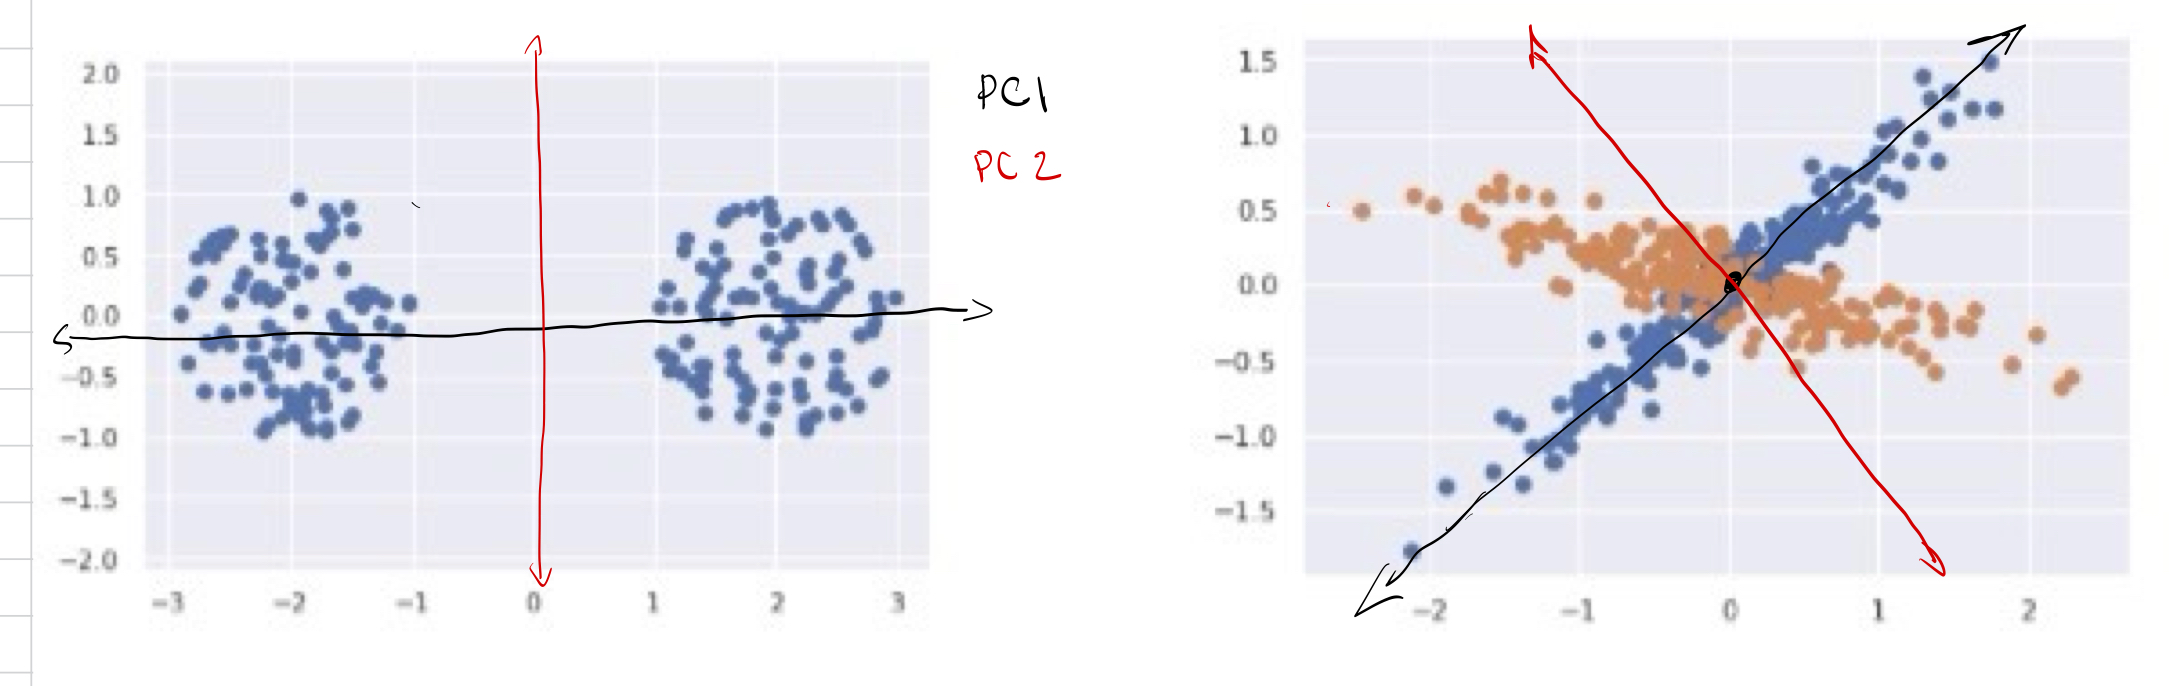
\includegraphics[width=0.75\textwidth]{1a.jpeg}
  \caption{PCA Components}
\end{figure}


\item If we want to retain $75\%$ of the variance, we would need to get the number of principal components that capture greater than $75\%$ of the sum of the covariance matrix eigenvalues. \\ 

The sum of the eigenvalues of the covariance matrix represent the total variance of the data and thus that computation is $2.1 + 1.8 + 1.3 + 0.9 + 0.4 + 0.2 + 0.15 + 0.02 + 0.001 = 6.871$. To retain $75\%$ of the variance, we would need to get the number of principal components that capture greater than $75\%$ of the sum of the covariance matrix eigenvalues. This would be $6.871 * 0.75 = 5.153$. \\ 

The largest amount of variance will be captured by the first components and the least number of components to get a sum greater than $5.153$ is $3$ components. $2.1 + 1.8 + 1.3 = 5.2$ \\ 

Therefore $K = 3$. 


\item \textbf{A}
\end{enumerate}

\item
\begin{enumerate}
\item To compute two iterations of the k-means algorithm we start with the following samples: \\ 

A = (2,3), B = (4,6), C = (5,1), and D = (10,12) \\ 
Our first initialized centroids are (6,9) for cluster 1 and (8,4) for cluster 2. \\


\textbf{Iteration 1: }\\ 

\begin{itemize}
\item A
  \begin{itemize}
    \item $d(A,1) = \sqrt((2-6)^2 + (3-9)^2) = \sqrt(52) = 7.211$ 
    \item $d(A,2) = \sqrt((2-8)^2 + (3-4)^2) = \sqrt(37) = 6.083$
  \end{itemize}

\item B 
  \begin{itemize}
    \item $d(B,1) = \sqrt((4-6)^2 + (6-9)^2) = \sqrt(13) = 3.606$
    \item $d(B,2) = \sqrt((4-8)^2 + (6-4)^2) = \sqrt(20) = 4.472$
  \end{itemize}
\item C
  \begin{itemize}
    \item $d(C,1) = \sqrt((5-6)^2 + (1-9)^2) = \sqrt(65) = 8.062$
    \item $d(C,2) = \sqrt((5-8)^2 + (1-4)^2) = \sqrt(18) = 4.243$
  \end{itemize}
\item D
  \begin{itemize}
    \item $d(D,1) = \sqrt((10-6)^2 + (12-9)^2) = \sqrt(25) = 5$
    \item $d(D,2) = \sqrt((10-8)^2 + (12-4)^2) = \sqrt(80) = 8.246$
  \end{itemize}
\item Cluster 1 members: B, D
\item Cluster 1 updated centroid = (7,9) \\ 
  updated centroid = midpoint(B,D) = ((4+10)/2, (6+12)/2) = (7,9)
\item Cluster 2 members: A, C \\ 
  updated centroid = midpoint(A,C) = ((2+5)/2, (3+1)/2) = (3.5,2) 
\end{itemize}

\textbf{Iteration 2: } \\ 

\begin{itemize}
  \item A
    \begin{itemize}
      \item $d(A,1) = \sqrt((2-7)^2 + (3-9)^2) = \sqrt(61) = 7.810$
      \item $d(A,2) = \sqrt((2-3.5)^2 + (3-2)^2) = \sqrt(3.25) = 1.803$
    \end{itemize}
  
  \item B 
    \begin{itemize}
      \item $d(B,1) = \sqrt((4-7)^2 + (6-9)^2) = \sqrt(18) = 4.243$
      \item $d(B,2) = \sqrt((4-3.5)^2 + (6-2)^2) = \sqrt(16.25) = 4.031$
    \end{itemize}
  \item C
    \begin{itemize}
      \item $d(C,1) = \sqrt((5-7)^2 + (1-9)^2) = \sqrt(68) = 8.246$
      \item $d(C,2) = \sqrt((5-3.5)^2 + (1-2)^2) = \sqrt(3.25) = 1.803$
    \end{itemize}
  \item D
    \begin{itemize}
      \item $d(D,1) = \sqrt((10-7)^2 + (12-9)^2) = \sqrt(18) = 4.243$
      \item $d(D,2) = \sqrt((10-3.5)^2 + (12-2)^2) = \sqrt(142.25) = 11.927$
    \end{itemize}
  \item Cluster 1 members: D
  \item Cluster 1 updated centroid = (10,12) \\ 
    updated centroid = midpoint(D) = (10,12)
  \item Cluster 2 members: A, B, C \\ 
    updated centroid = midpoint(A,B,C) = ((2+4+5)/3, (3+6+1)/3) = (3.67,3.33)
  \end{itemize}
\end{enumerate}

\item
  \begin{enumerate}
  \item \textbf{B}
  
  Since the output of the first filter will just simply be the sum of all the pixels weighted by 1/9, we can expect that the filter's behavior is that of an averaging over the 8 neighboring pixels and the pixel itself. This will result in a blurring effect because
  sharper parts of the image will be averaged out with the surrounding pixels. The image generally looks 'smoother' than it did before the filter was applied.
  \item \textbf{A}
    
  The kernel itself is all zeroes except for the center, which is 2. This means that for every kernel application, the output will double the pixel value of the center pixel. This generally means that when the filter is applied across the image, the image will be brighter across the entire image. 


  \item \textbf{C}
  
  When applying the kernel we noticed that it is darkening the image and also capturing a vertical line pattern. 
  \end{enumerate}

\item
  \begin{enumerate}
  \item \textbf{27} output size dimension 1

  To solve this problem, we will need two equations that help us reduce and count the dimension reduction/shift between convolutional layers. \\ 

  Given a convolutinal layer with kernel size $k x k$, stride $s$, and padding $p$, the output size $O$ of the output feature map for a given input dimension $D$ is going to be $O = \frac{D - k + 2 \cdot p}{s} + 1$. \\ 
  Furthermore, given a max pooling layer with kernel size $k x k$, stride $s$, and padding $p$, the output size $O$ of the output feature map for a given input dimension $D$ is going to be $O = \frac{D - k + 2 \cdot p}{s} + 1$. \\
  For a third feature, the number of out channels will be the dimension output of the previous layer. \\ 

  With these, we can compute the output size of the convolutional layers and the max pooling layers. \\ 
  Our network has 4 2d convolution layers and 3 max pool layers.

  We can progress through the network and compute the output size of each layer. We are given input size (232, 232, 3), dimensions 1, 2, 3 respectively \\ 
  \begin{itemize}
    \item Convolution layer 1: (In channels 3, Out channels 5, kernel: 5x5 Stride 1, Padding 0)\\ 
      \begin{itemize}
        \item $O_{\text{dimension}_1} = \frac{232 - 5 + 2 \cdot 0}{1} + 1 = 228$ 
        \item$O_{\text{dimension}_2} = \frac{232 - 5 + 2 \cdot 0}{1} + 1 = 228$ 
        \item $O_{\text{dimension}_3} = 5$ 
      \end{itemize}

    \item Max Pooling layer 1: (kernel: 2x2, Stride 2, Padding 0)\\ 
      \begin{itemize}
        \item $O_{\text{dimension}_1} = \frac{228 - 2 + 2 \cdot 0}{2} + 1 = 114$ 
        \item $O_{\text{dimension}_2} = \frac{228 - 2 + 2 \cdot 0}{2} + 1 = 114$ 
        \item $O_{\text{dimension}_3} = 5$ 
      \end{itemize}
    \item Convolution layer 2: (In channels 5, Out channels 10, kernel: 3x3, Stride 1, Padding 0)
      \begin{itemize}
        \item $O_{\text{dimension}_1} = \frac{114 - 3 + 2 \cdot 0}{1} + 1 = 112$ 
        \item $O_{\text{dimension}_2} = \frac{114 - 3 + 2 \cdot 0}{1} + 1 = 112$ 
        \item $O_{\text{dimension}_3} = 10$ 
      \end{itemize}
    \item Max Pooling layer 2: (kernel: 2x2, Stride 2, Padding 0)
      \begin{itemize}
        \item $O_{\text{dimension}_1} = \frac{112 - 2 + 2 \cdot 0}{2} + 1 = 56$ 
        \item $O_{\text{dimension}_2} = \frac{112 - 2 + 2 \cdot 0}{2} + 1 = 56$ 
        \item $O_{\text{dimension}_3} = 10$ 
      \end{itemize}
    \item Convolution layer 3: (In channels 10, Out channels 20, kernel: 3x3, Stride 1, Padding 0)
      \begin{itemize}
        \item $O_{\text{dimension}_1} = \frac{56 - 3 + 2 \cdot 0}{1} + 1 = 54$ 
        \item $O_{\text{dimension}_2} = \frac{56 - 3 + 2 \cdot 0}{1} + 1 = 54$ 
        \item $O_{\text{dimension}_3} = 20$ 
      \end{itemize}
    \item Max Pooling layer 3: (kernel: 2x2, Stride 2, Padding 0)
      \begin{itemize}
        \item $O_{\text{dimension}_1} = \frac{54 - 2 + 2 \cdot 0}{2} + 1 = 27$ 
        \item $O_{\text{dimension}_2} = \frac{54 - 2 + 2 \cdot 0}{2} + 1 = 27$ 
        \item $O_{\text{dimension}_3} = 20$ 
      \end{itemize}
  \end{itemize}

  We come to the conclusion of the output size of the network: (27, 27, 20).
  \item \textbf{27} output size dimension 2 
  \item \textbf{20} output size dimension 3
  \item \textbf{2660} total number of parameters

  Given the $C_{\text{out}}$, or number of output channels, number of input channels $C_{\text{in}}$, the kernel size $k x k$, we know the number of parameters 
  per convolutional layer is going to be $(C_{\text{out}} \cdot C_{\text{in}} \cdot k^2) + C_{\text{out}}$. \\

  We can compute the number of parameters for each layer and then sum them up \\ 
  \begin{itemize}
    \item Convolutional layer 1: $(5 \cdot 3 \cdot 5^2) + 5 = 380$
    \item Convolutional layer 2: $(10 \cdot 5 \cdot 3^2) + 10 = 460$
    \item Convolutional layer 3: $(20 \cdot 10 \cdot 3^2) + 20 = 1820$
  \end{itemize}

  Total parameters = 380 + 460 + 1820 = 2660

  \end{enumerate}
\end{enumerate}

\section{Python Programming Questions}

\begin{enumerate}
  \item \textbf{Question 1}
  \begin{enumerate}
    \item \textbf{1.4}
      \begin{figure}[H]
        \centering 
        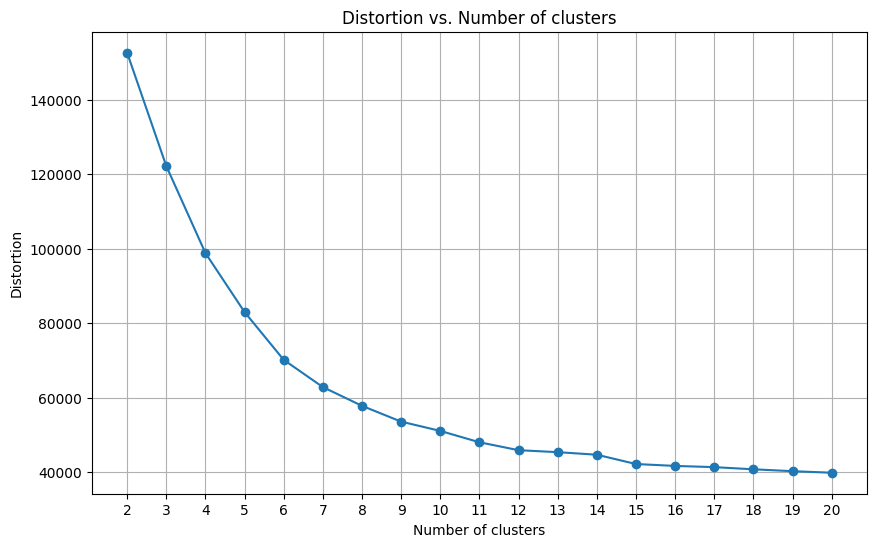
\includegraphics[width=0.75\textwidth]{1_4.png}
        \caption{K Means Clustering Elbow Method No Scaling}
      \end{figure}

      We can see the optimal k is somewhere between 7 and 8. Let us say k = 7. 
    \item \textbf{1.5}
    
    \begin{figure}[H]
      \centering 
      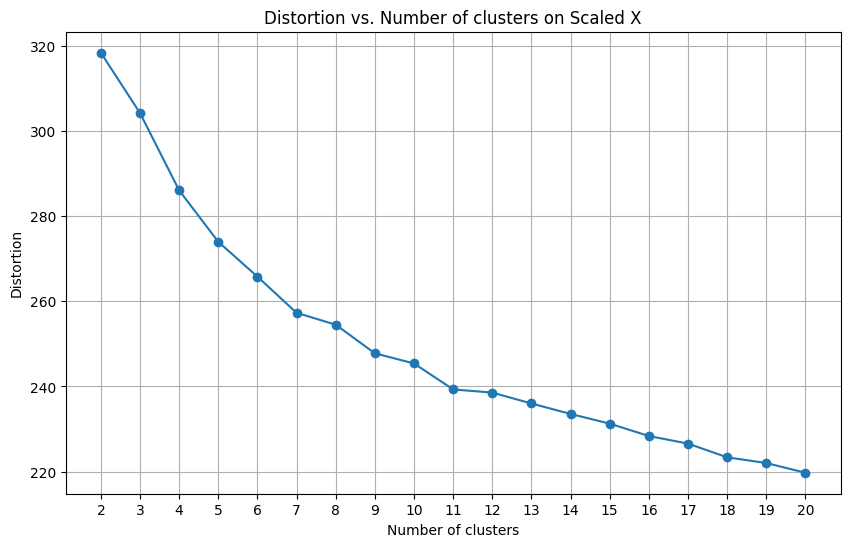
\includegraphics[width=0.75\textwidth]{1_5.png}
      \caption{K Means Clustering Elbow Method With Scaling}
    \end{figure}

    We can see the optimal k is somewhere between 10 and 11. Let us say k = 10. 

    \item \textbf{1.6}
    
    1. Why do you get different results with and without feature scaling? \\ 

    With feature scaling, the data is normalized to have a mean of 0 and a standard deviation of 1. This means that all the features are on the same numerical scale. This is important because now we are able to capture the distances between points on a uniform scale. Since we are less able to determine the clusters with the scaled data, we can see that the elbow method
    yields k = 10 or k = 11 as the optimal k. However, with the unscaled features, we notice that the elbow method yields an optimal k of k = 7 or k = 8. With the scaled features, we can see that we obtain a greater estimate for optimal k. The optimal k shifts because the focus of the features is distributed equally across all features. \\


    2. Should you scale the features before fitting k-means? Why or why not? \\

    Scaling the features is beneficial before fitting k-means clustering because we can capture the contributions of all features equally on the same scale. Thus, larger scale features will not overtake the algorithm, as we will have more accurate attribution and distance metric calculations. 
  

  \end{enumerate}

  \item \textbf{Question 2}
  \begin{enumerate}
    \item \textbf{2.1}
    \begin{figure}[H]
      \centering 
      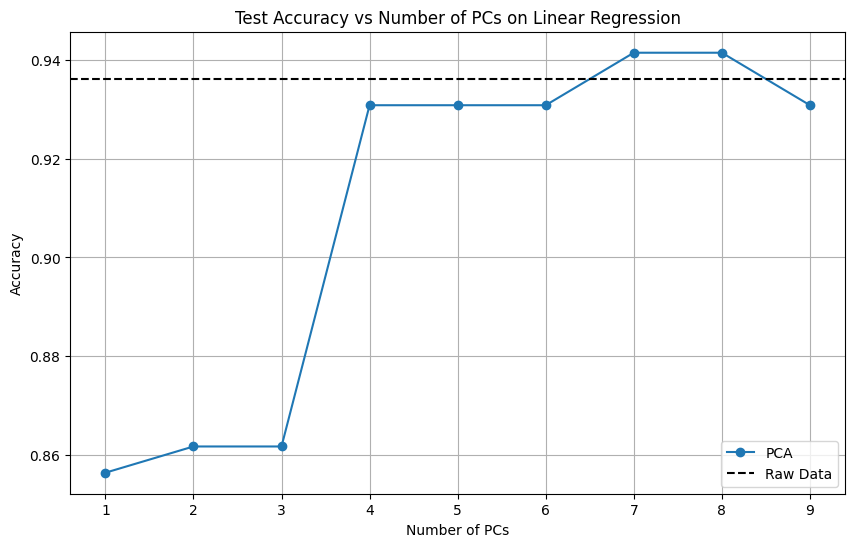
\includegraphics[width=0.75\textwidth]{2_1.png}
      \caption{PCA Accuracy}
    \end{figure}

    As expected, as we begin to add principal components to the model, the test accuracy of the model increases. However, after peaking at the 7th principal component, the test accuracy begins to level out and decreases slightly. This trend that we
    are noticing can be attributed to the fact that the model is overfitting to the training data. The model is capturing the noise in the data after the 7th principal component and thus the test accuracy begins to decrease. We also notice that
    adding principal components is not necessarily outperforming the original model without PCA. This could be due to the fact that the model itself already is attributing large weights to important features. 
    \item \textbf{2.2.2}
      The features that are explained best by the PCs together are 'Worst Area', 'Mean Area', and 'Area error'. Respectively, the explained variance by the PC's for 
      these three features are 0.852, 0.517, and 0.056. 
    \item \textbf{2.3}

    \begin{figure}[H]
      \centering 
      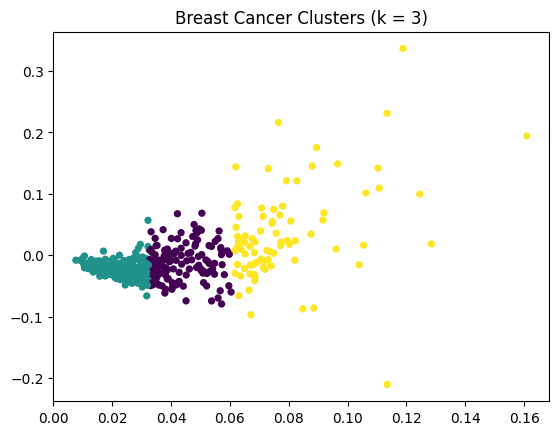
\includegraphics[width=0.75\textwidth]{2_3_3.png}
      \caption{Breast Cancer Clusters K = 3}
    \end{figure}

    \begin{figure}[H]
      \centering 
      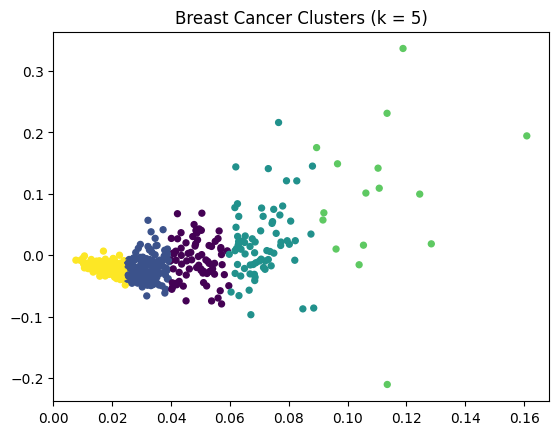
\includegraphics[width=0.75\textwidth]{2_3_5.png}
      \caption{Breast Cancer Clusters K = 5}
    \end{figure}

    \begin{figure}[H]
      \centering 
      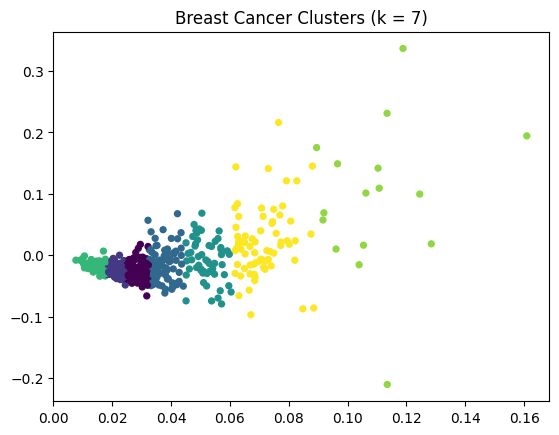
\includegraphics[width=0.75\textwidth]{2_3_7.png}
      \caption{Breast Cancer Clusters K = 7}
    \end{figure}

    \begin{figure}[H]
      \centering 
      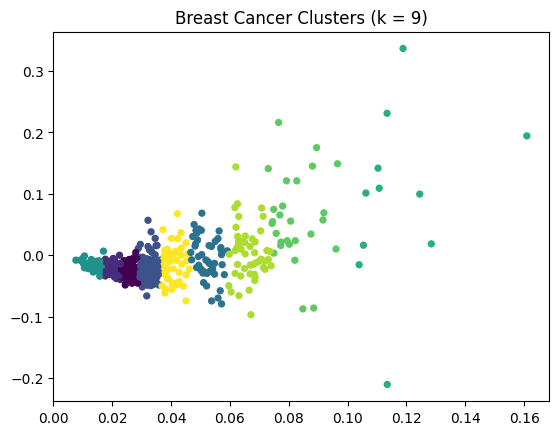
\includegraphics[width=0.75\textwidth]{2_3_9.png}
      \caption{Breast Cancer Clusters K = 9}
    \end{figure}

    \begin{figure}[H]
      \centering 
      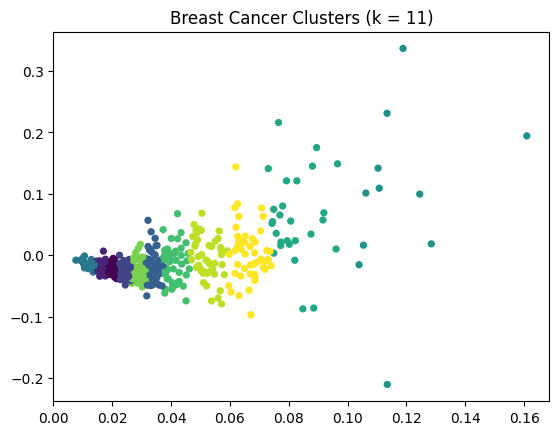
\includegraphics[width=0.75\textwidth]{2_3_11.png}
      \caption{Breast Cancer Clusters K = 11}
    \end{figure}

    For these figures, the greater the number k grows, the clusters will become more distinct. Especially for the wider part of the graph, we see that this entire part becomes distinct clusters as k grows. 


  \end{enumerate}


\end{enumerate}

% Complete questions in your iPython notebook and place all results here.

\end{document} 